\documentclass[a4paper]{article}

%% Language and font encodings
\usepackage[brazil]{babel}
\usepackage[utf8x]{inputenc}
\usepackage[T1]{fontenc}

%% Sets page size and margins
\usepackage[a4paper,top=3cm,bottom=2cm,left=3cm,right=3cm,marginparwidth=1.75cm]{geometry}

%% Useful packages
\usepackage{graphicx}
\usepackage{float}
\usepackage[colorinlistoftodos]{todonotes}
\usepackage[colorlinks=true, allcolors=blue]{hyperref}

\title{IF793 - Projeto Implementação de Jogos 2D}
\author{Luana Porciuncula Barreto}

\begin{document}
\maketitle

\begin{figure}[h]
	\centering
	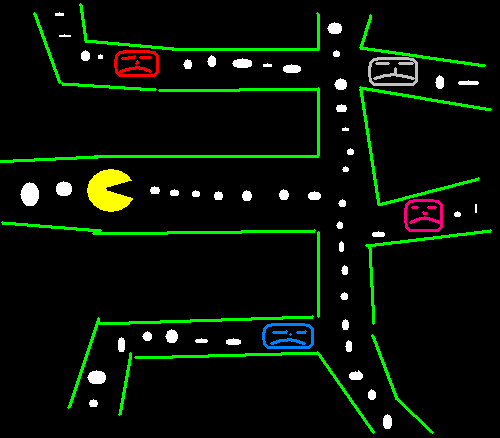
\includegraphics[width=0.3\textwidth]{lpb1.PNG}
\end{figure}

% * <lpb@cin.ufpe.br> 2018-05-07T00:36:00.983Z:
% 
% URL : https://commons.wikimedia.org/wiki/File:Pacman.PNG
% Autor: Wikibär
% Licença: Creative Commons Attribution-Share Alike 3.0 Unported
% 
% ^.

\section{Introdução}

Esta é uma disciplina eletiva que busca ambientar os alunos de Ciência da Computação da UFPE com as ferramentas, técnicas e conceitos de projeto e implementação de jogos. A matéria cobre brevemente a história e categorias de jogos, e foca em um projeto de jogo, iniciado desde o primeiro dia de aula, envolvendo tipo de jogo, tema, roteiro, contexto, personagens, interface, programação, arte gráfica e sonora, etc. A cadeira também envolve a aprendizagem  sobre ferramentas e bibliotecas (DirectX, XNA, J2ME) e de conceitos gráficos (Sprites, animação 3D, Modelo 2D e modelagem), sonoros, inteligência artificial e redes.

\begin{itemize}
	\item \cite{CinGame}Site da disciplina:\href{http://www.cin.ufpe.br/~game/}{~game}
	\item Material bibliográfico da cadeira:
    
	\begin{itemize}
    
		\item \cite{gamasutra} \href{http://www.gamasutra.com/}{Gamasutra}
        \item \cite{gameArchitecture} Game Architecture and Design
        \item \cite{gameDevMagazine} Game Developer Magazine
        \item \cite{gameproggemsSeries} Game Programming Gems Series
        \item \cite{gamedevSite} \href{https://www.gamedev.net/}{Gamedev}
        \item \cite{Rulesplay} Rules of Play : Game Design Fundamentals
        \item \cite{FunGameDesign} A Theory of Fun for Game Design
        \item \cite{AIWisdom} AI Game Programming Wisdom I, II, III
        
        
	\end{itemize}
    
\end{itemize}

\section{Relevância}

Devido à crescente área de influência dos aplicativos de entretenimento no mercado, torna-se óbvia a necessidade da disciplina Projeto Implementação de jogos no curso de Ciência da Computação. Além disso, ela exercita inter-disciplinaridade e tem relação direta com o mercado de trabalho atual. Ela tem como principais pontos positivos:

\begin{enumerate}
	\item Exercitar o imaginário e a criatividade.
	\item Ampliar os conhecimentos sobre interatividade, comunidade e produto.
	\item Proporcionar um desafio acadêmico, necessitando de conhecimentos de diversas áreas dentro e fora da computação.
\end{enumerate}

\section{Relação com outras disciplinas}

\begin{table}[h]
	\centering
	\caption{Disciplina | Relação}
	\begin{tabular}{cl}
		\hline
		\multicolumn{1}{|c|}{\begin{tabular}[c]{@{}c@{}}IF680 — Processamento Gráfico e \\ IF750 — Computação Gráfica\end{tabular}}     & \multicolumn{1}{l|}{\begin{tabular}[c]{@{}l@{}}As noções de computação gráfica, processamento de imagens\\ e visão computacional ensinadas nessas cadeiras são essenciais \\ para o design de uma arte gráfica do projeto do jogo.\end{tabular}}                                           \\ \hline
		\multicolumn{1}{|c|}{\begin{tabular}[c]{@{}c@{}}IF684 — Sistemas Inteligentes e\\ IF699 — Aprendizagem de Máquina\end{tabular}} & \multicolumn{1}{l|}{\begin{tabular}[c]{@{}l@{}}Projetos de jogos com roteiro mais complexos, normalmente\\  necessitam dos conhecimentos dessas cadeiras para\\ tornar a interação com outros personagens (NPCs, inimigos, etc)\\ mais realistas e aprimorar a jogabilidade.\end{tabular}} \\ \hline
		\multicolumn{1}{|c|}{IF687 — Introdução à Multimídia}                                                                           & \multicolumn{1}{l|}{\begin{tabular}[c]{@{}l@{}}Realidade virtual e realidade aumentada são duas noções cobertas\\ pela cadeira que são amplamente exploradas em jogos atualmente.\end{tabular}}                                                                                            \\ \hline
		\multicolumn{1}{|c|}{IF669 — Introdução à Programação}                                                                          & \multicolumn{1}{l|}{\begin{tabular}[c]{@{}l@{}}O projeto de um jogo envolve que o aluno tenha domínio dos\\ fundamentos da programação.\end{tabular}}                                                                                                                              \\ \hline
		\multicolumn{1}{|c|}{IF681 — Interfaces Usuário-Máquina}                                                                        & \multicolumn{1}{l|}{\begin{tabular}[c]{@{}l@{}}Os conceitos aprendidos nessa cadeira colaboram para criar uma \\ interface agradável no jogo, essencial para uma boa jogabilidade.\end{tabular}}                                                                                           \\ \hline
		\multicolumn{1}{l}{}                                                                                                            &                                                                                                                                                                                                                                                                                           
	\end{tabular}
\end{table}





\bibliographystyle{plain}
\bibliography{lpb}

\end{document}